\documentclass[serif,mathserif,final]{beamer}
\mode<presentation>{\usetheme{Lankton}}
\usepackage{amsmath,amsfonts,amssymb,pxfonts,eulervm,xspace,epstopdf}
\usepackage{graphicx}
\usepackage{amssymb}


\usepackage{graphicx} % Allows including images
\usepackage{booktabs} % Allows the use of \toprule, \midrule and \bottomrule in tables
\usepackage{epstopdf} % Allows to view .eps files
\usepackage{amsmath}
\usepackage{amssymb}
\usepackage{color}


\graphicspath{{./figures/}}
\usepackage [orientation=landscape,size=a1,scale=.8, debug]{beamerposter}
%[orientation=landscape,size=custom,width=84.1,height=59.4,scale=.8,debug]{beamerposter}
%[orientation=landscape,size=a1,scale=.8, debug]{beamerposter}

%-- Header and footer information ----------------------------------
\newcommand{\footleft}{http://staffwww.dcs.sheffield.ac.uk/people/M.Rahman/}
\newcommand{\footright}{M.Rahman@dcs.shef.ac.uk}

\title{A Probabilistic Dynamic Model for Transcription Factor Activity of C. Elegans}
\author{Muhammad Arifur Rahman, Prof. Neil D. Lawrence}
\institute{Sheffield Institute for Translational Neuroscience \\ The University of Sheffield, UK}
%-------------------------------------------------------------------


%-- Main Document --------------------------------------------------
\begin{document}
\begin{frame}{}
  \begin{columns}[t]

    %--------------------------------------------------------------------------------------------
    %--------------------------------------------------------------------------------------------
    %------------------------------- Column 1 ---------------------------------------------------
    %--------------------------------------------------------------------------------------------
    %--------------------------------------------------------------------------------------------
  

    \begin{column}{0.24\linewidth}

      %-- Block 1-1
      %--------------------------------------------------------------------------------------------
      \begin{block}{Motivation}
        
        \begin{itemize}

	  \item In molecular biology and genetics, a transcription factor is a protein that binds to specific DNA sequence.
	  \item Transcription factors control the flow (or transcription) of genetic information from DNA to mRNA. 
	  \item To develop models of cellular processes quantitative estimation of the regulatory relationship between transcription factors and genes is a basic requirement. 
	  \item It is difficult for a number of reasons: transcription factors’ expression levels are often low and noisy, and many transcription factors are post- transcriptionally regulated. 
	  \item So, from the expression levels of their target genes it is functional to infer the activity of the transcription factors.

	\end{itemize}
        
      \end{block}

      %-- Block 1-2
      %--------------------------------------------------------------------------------------------
      \begin{block}{C. Elegans}

	\begin{columns}[c] % The "c" option specifies centered vertical alignment while the "t" option is used for top vertical alignment

	\column{.45\textwidth} % Left column and width
	%\textbf{Some basic features-}
	\begin{itemize}
	\item Sydney Brenner (1927 - ) established C. Elegans as a model organism to study genetics and cell development.
	\item Adults are ~1mm long.
	\item They can be grown on agar plates with lawn of bacteria.
	\item They have a short generation time- 3 days from egg-laying to adulthood. 
	\item {Number of eukaryotic cells \color{green}$ \sim $ 1000} 
	
	\end{itemize}

	\column{.5\textwidth} % Right column and width
	\begin{itemize}
	\item {Number of neurons \color{green} $ \sim $ 300} 
	\item {Number of genes \color{red} $ \sim $ 15,139} \footnote{http://www.functionalnet.org/\\wormnet/about.html}
	\item {Number of Transcription factors \color{red} $ \sim $ 940} \footnote{ http://edgedb.umassmed.edu/\\TFFilesListingAction.do}
	\end{itemize}

	\begin{figure}[!htb]
	\centering
	\includegraphics[scale=.4]{picture/celegans_image2.jpg}
	% 1. http://www.stlawu.edu/news/bios/node/25
	% 2. http://bestcurrentaffairs.com/w/2013/04/28/genetic-code-of-panagrellus-redivivus-produced/
	\caption{C. Elegans}
	\label{fig:cElegans}
	\end{figure}

	\end{columns}

      \end{block}

      %-- Block 1-3
      %--------------------------------------------------------------------------------------------
      \begin{block}{Transcription}
       
	  \begin{columns}[c] % The "c" option specifies centered vertical alignment while the "t" option is used for top vertical alignment
	  \column{.45\textwidth} % Left column and width
	  %\textbf{Some basic features-}
	  \begin{itemize}
	  \item The information in DNA is not directly converted into proteins, but must first be copied into RNA
	  \item Transcription produces genetic messages in the form of mRNA.
	  \item During transcription, a DNA sequence is read by an RNA polymerase. 
	  \item Transcription produces a complementary, anti-parallel RNA strand
	  \end{itemize}

	  \column{.5\textwidth} % Right column and width

	  \begin{figure}[!htb]
	  \centering
	  \includegraphics[scale=.18]{picture/Transcription.png}
	  % Copyright 2003: Pearson Education, Inc. publishing as Benjamin Cummings
	  \caption{Transcription \footnote{Copyright 2003: Pearson Education, Inc. \\ publishing as Benjamin Cummings}}
	  \label{fig:transcription}
	  \end{figure}

	  \end{columns}
       
      \end{block}

      %-- Block 1-4
      %--------------------------------------------------------------------------------------------
     \begin{block}{Method}
	  Our basic approach follows a dynamic model that extends the linear 
	  regression model of  \cite{p1}  and 
	  probabilistic model of  \cite{p2} to model the distribution 
	  of each transcription factor acting on each gene.
       
      \end{block}
    
      
    \end{column}%1


    %--------------------------------------------------------------------------------------------
    %--------------------------------------------------------------------------------------------
    %------------------------------- Column 2 ---------------------------------------------------
    %--------------------------------------------------------------------------------------------
    %--------------------------------------------------------------------------------------------
    
    \begin{column}{0.24\linewidth}

      %-- Block 2-1
      %--------------------------------------------------------------------------------------------
      \begin{block}{Transcription Process}
      
	  \begin{columns}[c] % The "c" option specifies centered vertical alignment while the "t" option is used for top vertical alignment

	  \column{.45\textwidth} % Left column and width
	  \textbf{Three main steps of transcription process-}
	  \begin{itemize}
	  \item {\bf Initiation} : Transcription process starts at the promoter region of a double-stranded DNA. 
	  \item {\bf Elongation} : A sequence specific DNA binding factors called transcription factors then unwind the DNA strand
	  \item {\bf Termination} : Unwinding DNA's double helical form RNA polymerase reaches the terminator sequence. Here, RNA polymerase releases the mRNA polymer.
	  \end{itemize}

	  \column{.5\textwidth} % Right column and width

	  \begin{figure}[!htb]
	  \centering
	  \includegraphics[scale=.5]{picture/transcriptionProcess.png}
	  % Copyright 2003: Pearson Education, Inc. publishing as Benjamin Cummings
	  %\caption{Transcription Process}
	  \label{fig:transcriptionProcess}
	  \end{figure}

	  \end{columns}
     
      \end{block}

      %-- Block 2-2
      %--------------------------------------------------------------------------------------------
      \begin{block}{Mapping between environmental signal and transcription factors on Genes}

      
	  \begin{figure}[!htb]
	  \centering
	  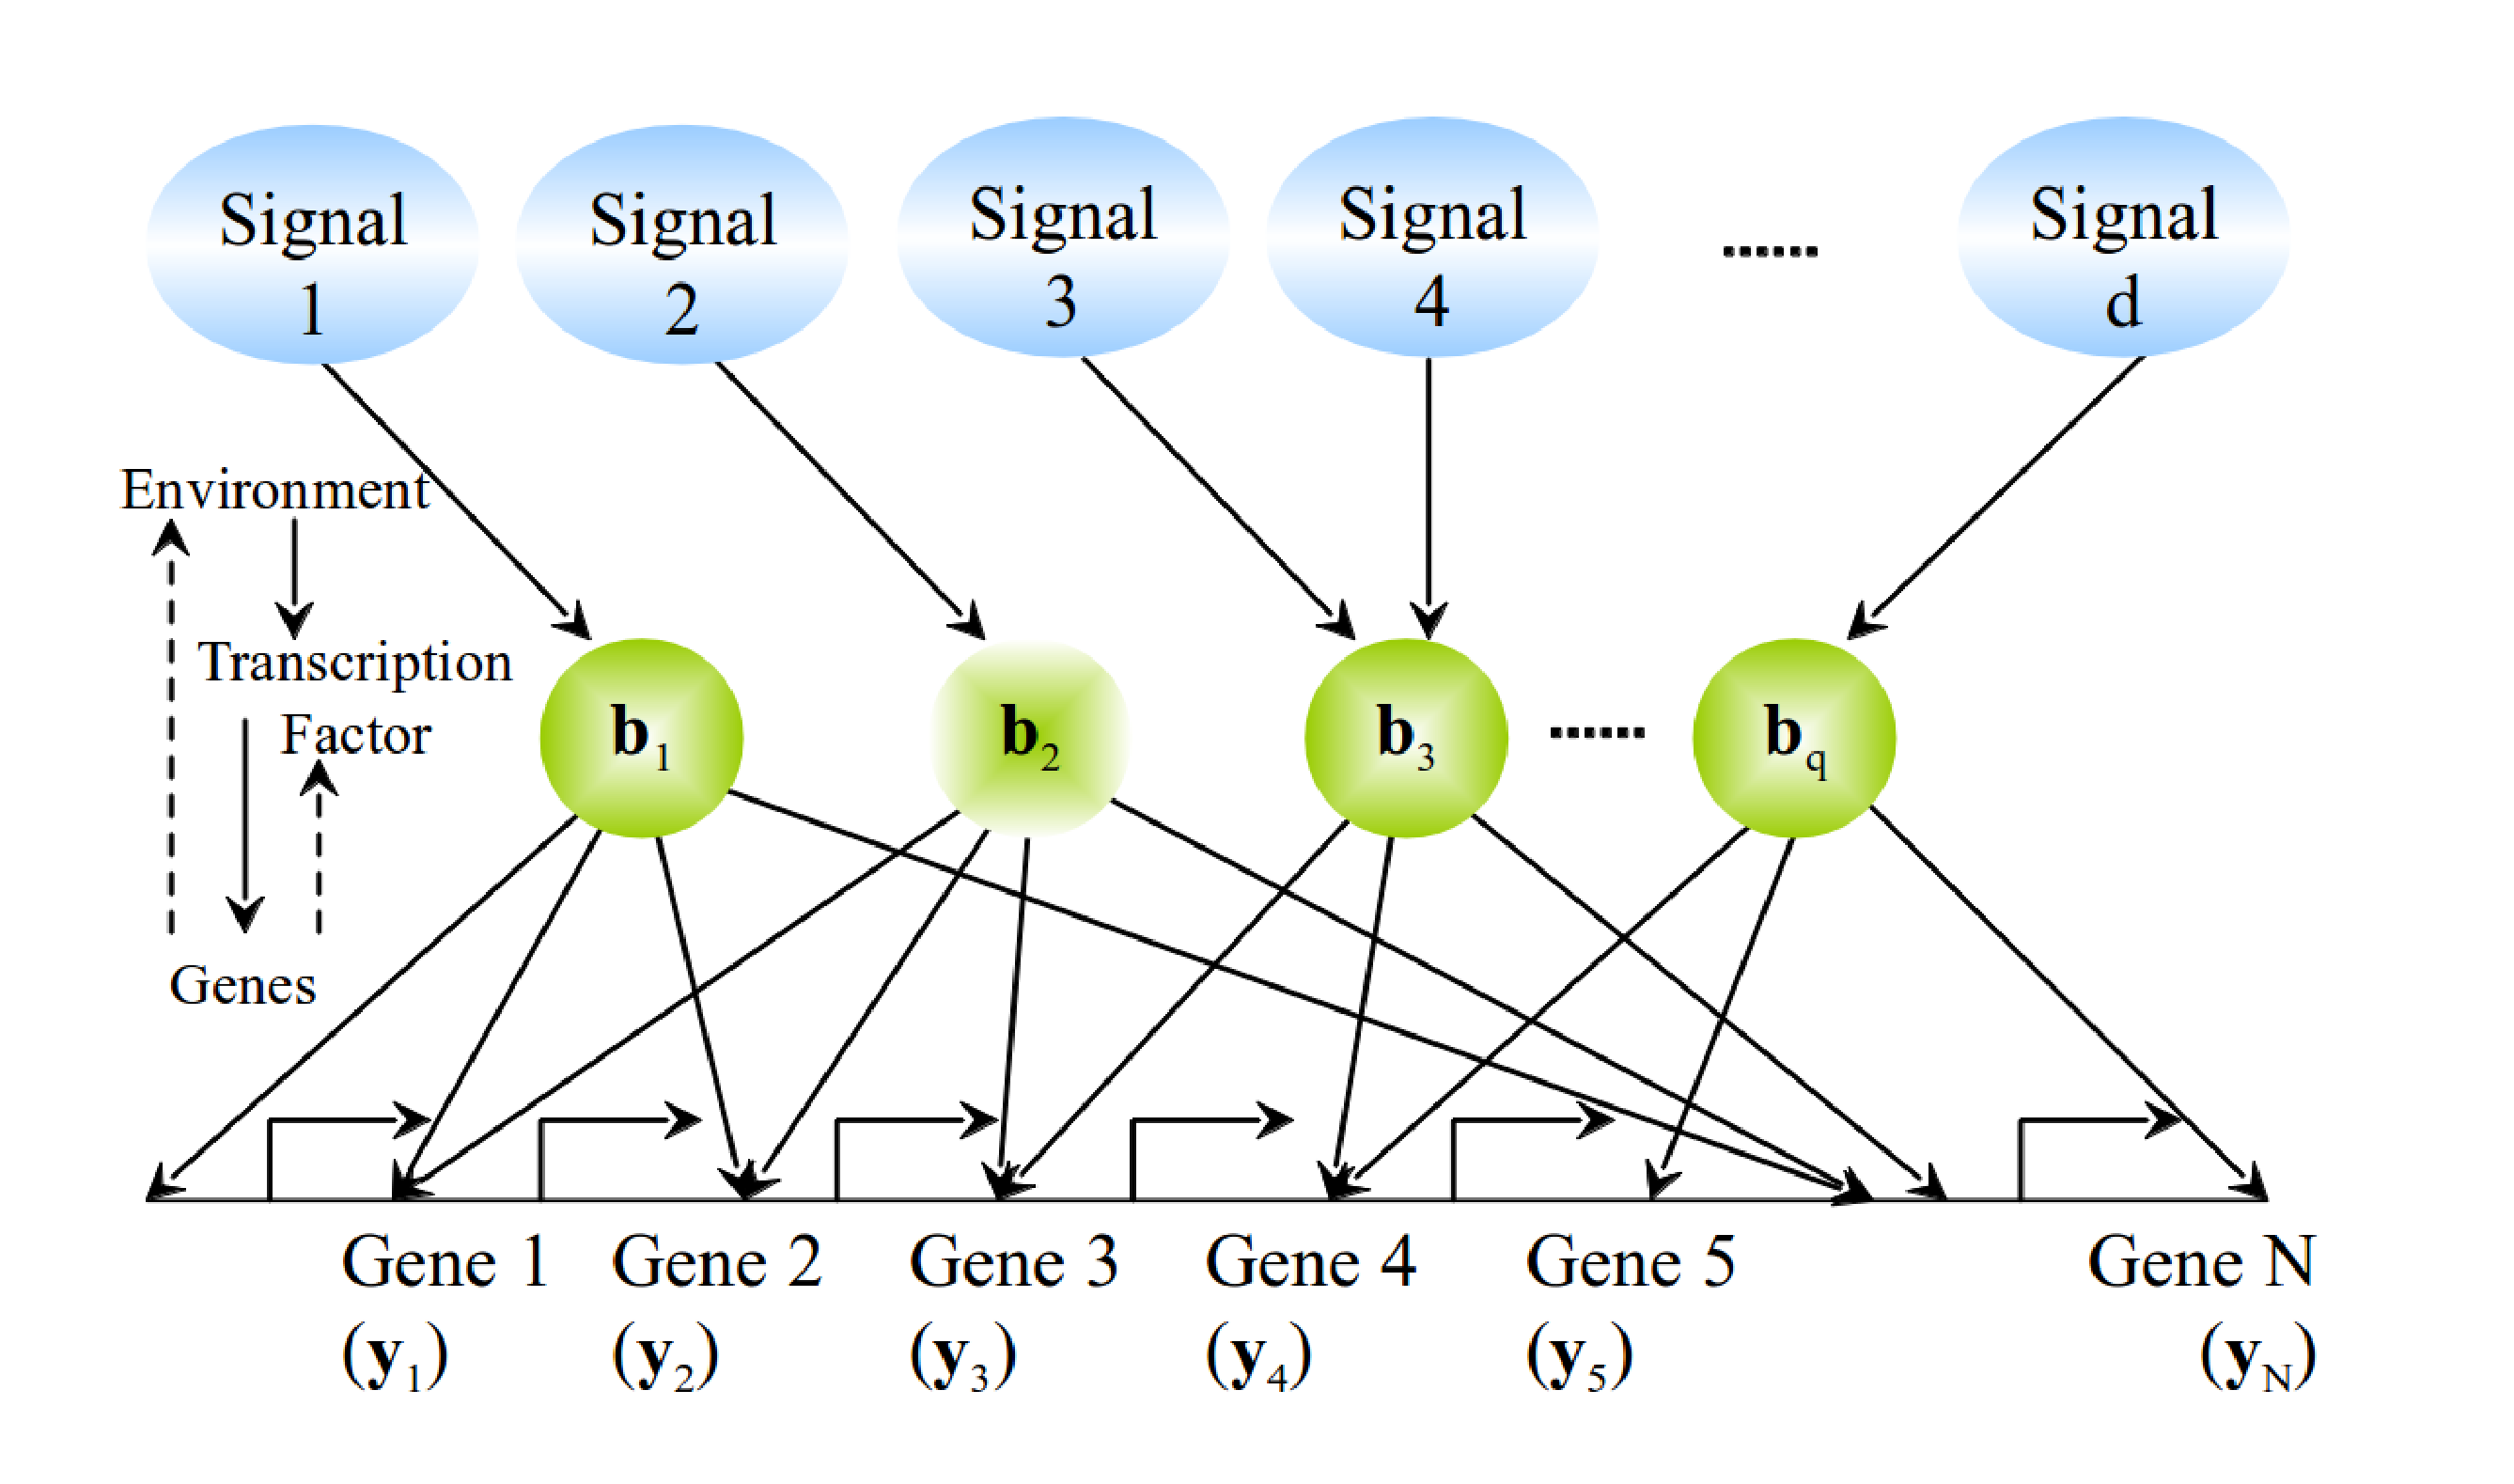
\includegraphics[scale=.43]{picture/signaltoTFA.eps}
	  %\caption{Mapping between environmental signal and transcription factors on Genes}
	  \label{fig: mapping }
	  \end{figure}
      
      
      \end{block}

      %-- Block 2-3
      %--------------------------------------------------------------------------------------------
      \begin{block}{Probabilistic Model}
	  Let, Gene expression- $ \bold{Y} \in \mathbb{R} ^ { \bold{N} \times \bold{d} } $ \\
	  Connectivity matrix- $ \bold{X} \in \mathbb{R} ^ { \bold{N} \times \bold{q} } $ \\

	  Based on Sanguinetti et al. (2006) TFAs can be obtained by regressing the gene expressions using the connectivity information, giving the following linear model- \\
	  \centering { $ \bold{y_{n}} = \bold{B_{n}} \bold{x_{n}} + \boldsymbol{\epsilon_{n}}$ } \\

	  Here $n = 1, . . . ,N$ indexes the gene, $ \bold{y_{n}} = \bold{Y}(n,:)^T $, $ \bold{x_{n}} = \bold{X}(n,:)^T $ and  $ \boldsymbol{\epsilon_{n}} $ is an error term. The matrix $ \bold{B_{n}} $ has $ d $ rows and $ q $ columns, and models the gene specific TFAs \\~\\
      
	Two plausible assumptions for TFA-
	\begin{itemize}
	\item Firstly, Gene specific TFA $ \bold{b}_{nt} $ at time $ t $ depends solely on the gene specific TFA at time $ (t-1) $. 
	\item Secondly, it was assumed that the prior distribution to be a stationary in time. \\~\\
	\end {itemize}
      
      \end{block}

      \end{column}%3


    %--------------------------------------------------------------------------------------------
    %--------------------------------------------------------------------------------------------
    %------------------------------- Column 3 ---------------------------------------------------
    %--------------------------------------------------------------------------------------------
    %--------------------------------------------------------------------------------------------
    
    
    \begin{column}{0.24\linewidth}

      %-- Block 3-1
      %--------------------------------------------------------------------------------------------
      \begin{block}{}

	Two limiting case-
	\begin{itemize}
	\item The first limiting case when all the $ \bold{b}_{nt} $ assumed to be identical, so that- \\
	\centering { $ \bold{b}_{n1} \sim \mathcal{N} ( \boldsymbol{\mu},\bold{\Sigma})$ and $ \bold{b}_{n(t+1)} \sim \mathcal{N} ( \bold{b}_{nt},\bold{0})$}
	%\raggedleft
	\raggedright
	\item Second limiting case was when all the $ \bold{ b_{nt}} $ were assumed to be independent and identically distributed- \\ \centering {$ \bold{b}_{nt} \sim \mathcal{N} ( \boldsymbol{\mu},\bold{\Sigma})$}

	\end{itemize}
      
	\begin{itemize}
	\item  \cite{p2}  expected a realistic model of time series data to be somewhere in between this two extremes- \\
	\centering $ \bold{b}_{n(t+1)} \sim \mathcal{N} (\gamma \bold{b}_{nt} + (1-\gamma)\boldsymbol{\mu},(1-\gamma^2)\bold{\Sigma})$ \\
	for $ t= 1, ... , (d-1)$ and $ \bold{b}_{n1} \sim \mathcal{N} ( \boldsymbol{\mu},\bold{\Sigma})$
	\raggedright
	\\ Where $ \gamma $ is a parameter measuring the degree of temporal continuity of the TFAs \\~\\

	\item Likelihood function-\\
	\centering 
	$p(\bold{Y|B,X})= \displaystyle \prod_{n \mathop = 1}^{N} p(\bold{y_n|B_n,x_n})$

	\raggedright
	\item TFAs can be estimated a posteriori using Bayes’s Theorem- \\~\\
	\centering 
	$ p(\bold{b_n|Y})= \frac {p(\bold{Y|b_n})p(\bold{b_n})}{p(\bold{Y})} $

	\end {itemize}
      
      \end{block}

      
      %-- Block 3-2
      %--------------------------------------------------------------------------------------------
      
      \begin{block}{Gene Specific TFA of T20B12.8}
    
      \begin{figure}
      \includegraphics[width=0.6\linewidth]{picture/T20B12_8_3.eps}
      %\caption{Gene Specific TFA of T20B12.8}
      \end{figure}

      \end{block}

      
      %-- Block 3-3
      %--------------------------------------------------------------------------------------------
      \begin{block}{Gene Specific TFA of ZK370.2}
      
      \begin{figure}
      \includegraphics[width=0.6\linewidth]{picture/ZK370_2_3.eps}
      %\caption{Gene Specific TFA of ZK370.2}
      \end{figure}

      \end{block}
       
            
    \end{column}%3

    %--------------------------------------------------------------------------------------------
    %--------------------------------------------------------------------------------------------
    %------------------------------- Column 4 ---------------------------------------------------
    %--------------------------------------------------------------------------------------------
    %--------------------------------------------------------------------------------------------
    
    \begin{column}{0.24\linewidth}

      
      %-- Block 4-1
      %--------------------------------------------------------------------------------------------
            \begin{block}{Genes regulated by multiple TF}
             
        \begin{table}
	  \begin{tabular}{l l }
	      \textbf{Gene Name} & \textbf{Regulators activity} \\
	      {\color{red}C44B12.5} & {\color{blue} Y116A8C.35 }= $ 1.719797 \pm 3.493205 $, \\ 
				    & {\color{blue}F33A8.3} = $ 1.415785 \pm 3.492985$ \\~\\

		{\color{red}Y105E8B.3} & {\color{blue} Y54G2A.1} = $ 0.07157665 \pm 1.2222137 $ \\
		  & {\color{blue} F33D11.12} = $ 0.03861905 \pm 0.7252534 $ \\
 		  & {\color{blue} ZK370.2} = $ -1.20157055 \pm  2.0318513 $\\~\\
		    
	      {\color{red} Y105E8B.3} & {\color{blue} T20B12.8 } = $ 0.25474933 \pm  2.5665869 $ \\
		  			& {\color{blue} F33A8.3 } = $ 0.11619828  \pm  3.5107742 $ \\
 		  			& {\color{blue} Y116A8C.35 } = $ 0.03289664 \pm  3.8071374 $ \\
					& {\color{blue} F11A10.2 } = $ 0.03016348 \pm 1.7737585 $ \\
 		  			& {\color{blue} C16A3.7  } = $ 0.01883489 \pm  $ 0.9431105\\

	  \end{tabular}
	  \caption{Genes regulated by multiple TF}
	  \end{table}
       
       \end{block}

       
      %-- Block 4-2
      %--------------------------------------------------------------------------------------------
      \begin{block}{Discussions}
	  \begin{itemize}
	  \item Most of the existing models infer transcription factor activities that are shared across gene. 
	  \item Here we infer the gene-specific transcription factor activities for C. Elegans. 
	  \item Genome-wide investigation could be possible.
	  \item We can also determine which regulations are significant for a given experimental condition.
	  \item To validate the new biological data these predictions could be very helpful.
	  \end{itemize}

      \end{block}

      %-- Block 4-3
      %--------------------------------------------------------------------------------------------
      \begin{block}{Acknowledgements}

      \begin{itemize}
      \item {\bf Prof. Andrew Cossins}, Institute of Integrative Biology, University of Liverpool for the data set and valuable suggestions. \\

      \item {\bf puma} : The Bioconductor package. \\

      \item {\bf Ministry of Science, Information and Communication Technology, Bangladesh} for funding the scholarship.

      \end{itemize}
      
      \end{block}

      %-- Block 4-4
      %--------------------------------------------------------------------------------------------
      \begin{block}{References}
                
	\footnotesize{
	\begin{thebibliography}{99} % Beamer does not support BibTeX so references must be inserted manually as below

	\bibitem[Lee et al. 2008]{p5} Lee I., Lehner B., Crombie C., Wang W., Fraser A G., and Marcotte E M. (2008)
	\newblock A single network comprising the majority of genes accurately predicts the phenotypic effects of gene perturbation in C. elegans
	\newblock \emph{Nature Genetics}, Vol 40, pages 181-188 
	
	\bibitem[Liao et al., 2003]{p1} Liao, J.C. Liao JC, Boscolo R, Yang YL, Tran LM, Sabatti C, Roychowdhury VP. (2003)
	\newblock Network component analysis: reconstruction of regulatory signals in biological systems.
	\newblock \emph{Proc Natl Acad Sci U S A.} 2003 Dec 23;100(26):15522-7. Epub 2003 Dec 12.

	\bibitem[Liu,X. et al. 2005]{p3} Liu X., Milo M., Lawrence N.D. and Rattray M. (2005) 
	\newblock A tractable probabilistic model for affymetrix probe-level analysis across multiple chips. 
	\newblock \emph {Bioinformatics}, 21, 3637–3644.

	\bibitem[Nachman,I. et al. 2004]{p4}Nachman I., Regev I., Friedman N. (2004) 
	\newblock Inferring quantitative models of regulatory networks from expression data. 
	\newblock \emph{Bioinformatics}, 20, i248–i256.

	\bibitem[Sanguinetti et al., 2006]{p2} Sanguinetti G, Rattray M., and Lawrence N.D. (2006)
	\newblock A probabilistic dynamical model for quantitative inference of the regulatory mechanism of transcription
	\newblock \emph{Bioinformatics, Oxford University Press}, Vol. 22 no. 14, pages 1753–1759 (2006)
	
	\end{thebibliography}
	}
                
      \end{block}

    \end{column}%4
    
  \end{columns}
\end{frame}
\end{document}
